\section{Phân tích chi tiết các kiến trúc phần mềm}

\begin{flushleft}
  \hspace*{0.8cm}Ba mô hình kiến trúc phần mềm phổ biến là kiến trúc ba tầng, MVC và MVVM đều hướng đến việc tổ chức mã nguồn rõ ràng, dễ bảo trì và mở rộng. Kiến trúc ba tầng chia hệ thống thành ba phần riêng biệt: trình diễn, nghiệp vụ và dữ liệu, giúp tăng tính độc lập giữa các tầng và phù hợp với các hệ thống có quy mô lớn. Trong khi đó, MVC tập trung vào việc tách biệt giao diện (View), dữ liệu (Model) và điều khiển (Controller), thường được sử dụng trong phát triển ứng dụng iOS với lợi thế trong việc hỗ trợ nhiều nhóm làm việc song song. MVVM, một phiên bản hiện đại hơn, thay Controller bằng ViewModel – giúp kết nối thông minh giữa View và Model thông qua Data Binding. Nhờ vậy, MVVM giảm sự phụ thuộc giữa các thành phần, tăng khả năng tự động hóa trong cập nhật giao diện và đặc biệt phù hợp với phát triển ứng dụng Android. Mỗi kiến trúc đều có ưu điểm riêng và được lựa chọn tùy thuộc vào nền tảng phát triển, quy mô hệ thống và yêu cầu kỹ thuật cụ thể.
  \end{flushleft}
  
  

% 4.1
\subsection{Kiến trúc phần mềm ba tầng (Three-tier architecture).}
\renewcommand{\labelitemi}{--}    
\begin{flushleft}
  \hspace*{0.8cm}Trong lĩnh vực phát triển phần mềm hiện đại, một trong những mô hình kiến trúc được áp dụng phổ biến và hiệu quả nhất chính là kiến trúc phần mềm ba tầng. Mô hình này đặc biệt phù hợp với các hệ thống quy mô lớn, có yêu cầu cao về tính bảo trì, khả năng mở rộng và dễ dàng tích hợp các công nghệ mới.
  \end{flushleft}
  
  \begin{flushleft}
  \hspace*{0.8cm}Kiến trúc ba tầng phân chia ứng dụng thành ba lớp riêng biệt, bao gồm: tầng trình diễn (Presentation Layer), tầng nghiệp vụ (Business Logic Layer) và tầng dữ liệu (Data Layer). Mỗi tầng này đảm nhận một vai trò cụ thể và được thiết kế để hoạt động độc lập, tuy nhiên vẫn giữ mối liên kết chặt chẽ với nhau thông qua các giao diện lập trình ứng dụng (API) hoặc các giao thức truyền thông nội bộ. Sự tách biệt này giúp nâng cao tính linh hoạt, giảm thiểu sự phụ thuộc giữa các phần và tạo điều kiện thuận lợi cho việc kiểm thử, phát triển song song cũng như tái sử dụng mã nguồn.
  \end{flushleft}

  % https://viquynh.wordpress.com/2018/02/05/mo-hinh-mvc2-code-demo-jsp-servlet-javabe/
\begin{figure}[H]
  \centering
  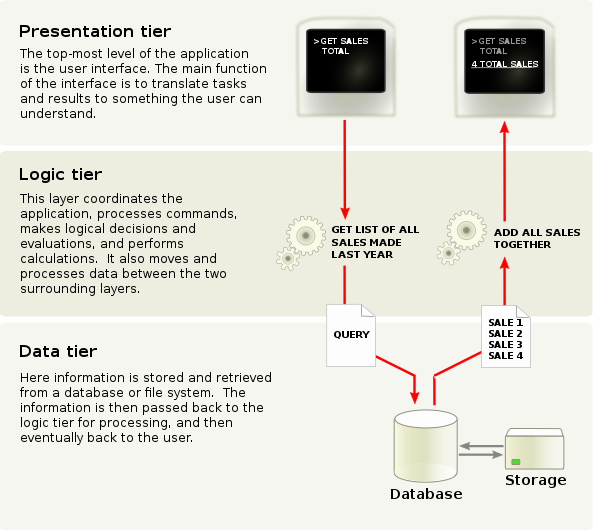
\includegraphics[width=0.75\textwidth]{images/layer.png}
  \caption{Mô hình kiến trúc 3 tầng (3-tiers) \cite{vneconomyNokia}.}
  \label{fig:15}
\end{figure}
  
  \begin{flushleft}
  \hspace*{0.8cm}Ở tầng cao nhất của kiến trúc, tầng trình diễn đóng vai trò là điểm tiếp xúc trực tiếp giữa người dùng và hệ thống phần mềm. Chức năng chính của tầng trình diễn là đảm nhận việc hiển thị thông tin đầu ra và nhận các dữ liệu đầu vào từ người dùng thông qua giao diện đồ họa hoặc giao diện điều khiển. Việc sử dụng các công nghệ như HTML, CSS, JavaScript trong các ứng dụng web hoặc framework giao diện trong ứng dụng mobile, cho phép tầng này cung cấp trải nghiệm người dùng mượt mà và trực quan.
  \end{flushleft}
  
  \begin{flushleft}
  \hspace*{0.8cm}Thông tin được hiển thị tại tầng giao diện không được xử lý trực tiếp tại đây mà được chuyển tiếp từ tầng nghiệp vụ đã xử lý sẵn. Điều này giúp giao diện người dùng trở nên đơn giản, linh hoạt và dễ dàng thay đổi mà không ảnh hưởng đến các tầng khác. Ví dụ, một chức năng tính toán giá sau khi áp dụng khuyến mãi sẽ được xử lý hoàn toàn ở tầng nghiệp vụ, và kết quả cuối cùng chỉ được hiển thị lên giao diện.
  \end{flushleft}
  
  \begin{flushleft}
  \hspace*{0.8cm}Sự phân tách này còn mang lại lợi thế lớn trong việc phát triển đa nền tảng. Khi cùng một logic nghiệp vụ có thể được dùng lại trên cả ứng dụng web và ứng dụng mobile, nhóm phát triển chỉ cần xây dựng lại giao diện riêng biệt cho từng nền tảng mà không cần viết lại phần xử lý chính bên trong.
  \end{flushleft}
  
  \begin{flushleft}
  \hspace*{0.8cm}Tầng thứ hai trong mô hình là tầng nghiệp vụ, đóng vai trò trung tâm và là nơi diễn ra toàn bộ quá trình xử lý logic của hệ thống. Tầng này là nơi hiện thực các quy tắc hoạt động của ứng dụng, như các thuật toán tính toán, kiểm tra ràng buộc dữ liệu, xử lý yêu cầu nghiệp vụ và điều phối luồng dữ liệu giữa các tầng.
  \end{flushleft}
  
  \begin{flushleft}
  \hspace*{0.8cm}Khi người dùng thực hiện một hành động từ tầng trình diễn, yêu cầu tương ứng sẽ được gửi tới tầng nghiệp vụ để phân tích và xử lý. Nếu cần thiết, tầng nghiệp vụ sẽ tiếp tục giao tiếp với tầng dữ liệu để truy xuất hoặc ghi nhận thông tin, sau đó định dạng kết quả và chuyển trả lại tầng giao diện. Cách tổ chức này giúp cô lập hoàn toàn các logic phức tạp, đảm bảo việc thay đổi giao diện hoặc cơ sở dữ liệu không làm ảnh hưởng đến phần cốt lõi của ứng dụng.
  \end{flushleft}
  
  \begin{flushleft}
  \hspace*{0.8cm}Một điểm nổi bật của tầng nghiệp vụ là khả năng hỗ trợ kiểm thử đơn vị (unit testing) dễ dàng hơn. Nhờ vào tính độc lập và không phụ thuộc vào giao diện người dùng hay cơ sở dữ liệu, các chức năng tại tầng nghiệp vụ có thể được kiểm thử tự động nhằm đảm bảo độ chính xác và tính ổn định lâu dài của hệ thống.
  \end{flushleft}
  
  \begin{flushleft}
  \hspace*{0.8cm}Tầng cuối cùng là tầng dữ liệu, chịu trách nhiệm quản lý và lưu trữ toàn bộ thông tin phục vụ cho hoạt động của hệ thống. Dữ liệu ở tầng này thường được tổ chức và xử lý thông qua các hệ quản trị cơ sở dữ liệu như MySQL, PostgreSQL, MongoDB hoặc các giải pháp lưu trữ đám mây như Firebase, Amazon S3.
  \end{flushleft}
  
  \begin{flushleft}
  \hspace*{0.8cm}Tầng dữ liệu cung cấp các cơ chế truy vấn, cập nhật, xoá và bảo mật dữ liệu một cách có hệ thống. Bên cạnh đó, tầng này cũng đảm nhiệm việc tối ưu hóa hiệu suất truy vấn và đảm bảo tính nhất quán dữ liệu thông qua các ràng buộc và transaction. Với các hệ thống có khối lượng dữ liệu lớn hoặc phải phục vụ nhiều người dùng đồng thời, việc thiết kế và tối ưu tầng dữ liệu trở thành yếu tố then chốt ảnh hưởng trực tiếp đến hiệu năng tổng thể.
  \end{flushleft}
  
  \begin{flushleft}
  \hspace*{0.8cm}Nhìn chung, kiến trúc phần mềm ba tầng cung cấp một khung tổ chức rõ ràng, trong đó mỗi tầng đóng một vai trò cụ thể nhưng hỗ trợ lẫn nhau nhằm đảm bảo tính ổn định, dễ bảo trì và dễ mở rộng cho hệ thống. Sự tách biệt về mặt chức năng giữa các tầng giúp nhóm phát triển có thể làm việc song song, dễ dàng kiểm thử từng phần riêng biệt và nhanh chóng thích ứng với các yêu cầu thay đổi từ khách hàng hoặc thị trường.
  \end{flushleft}
  
  \begin{flushleft}
  \hspace*{0.8cm}Với những lợi ích nổi bật đó, kiến trúc ba tầng đã trở thành sự lựa chọn phổ biến trong nhiều lĩnh vực, từ các ứng dụng doanh nghiệp nội bộ, hệ thống thương mại điện tử, đến các nền tảng dịch vụ trực tuyến lớn như hệ thống ngân hàng, cổng thanh toán điện tử hay hệ thống quản lý chuỗi cung ứng.
  \end{flushleft}

% 4.2
\subsection{Kiến trúc MVC (Model – View – Controller)}
\renewcommand{\labelitemi}{--}    
    \begin{flushleft}
        \hspace*{0.8cm}Trong quá trình phát triển phần mềm, đặc biệt là trong các ứng dụng di động trên nền tảng iOS, kiến trúc MVC (Model – View – Controller) đóng vai trò như một nền tảng tổ chức mã nguồn kinh điển, giúp lập trình viên tách biệt các chức năng chính của ứng dụng thành ba phần riêng biệt.
    \end{flushleft}

        % https://daynhauhoc.com/t/loi-load-du-lieu-len-jsp/109965/10
\begin{figure}[H]
  \centering
  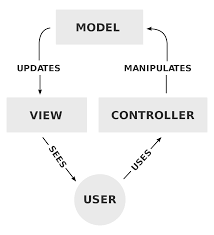
\includegraphics[width=0.5\textwidth]{images/mvc.png}
  \caption{Mô hình kiến trúc MVC \cite{daynhauhocMVC}.}
  \label{fig:fig19}
\end{figure}

    \begin{flushleft}
      \hspace*{0.8cm}Việc phân chia này không chỉ nhằm giảm độ phức tạp của hệ thống mà còn tạo điều kiện thuận lợi cho quá trình bảo trì, kiểm thử và mở rộng về sau. Theo mô hình này, toàn bộ hệ thống được chia thành ba thành phần chính: Model (xử lý dữ liệu và logic nghiệp vụ), View (hiển thị giao diện người dùng), và Controller (điều phối luồng xử lý giữa Model và View). Mỗi thành phần trong ba thành phần này đảm nhiệm một vai trò cụ thể và độc lập, tuy nhiên lại phối hợp chặt chẽ để tạo nên một hệ thống vận hành ổn định và linh hoạt.
    \end{flushleft}

    \begin{flushleft}
      \hspace*{0.8cm}Với vai trò là trung tâm lưu trữ dữ liệu, thành phần Model trong kiến trúc MVC chịu trách nhiệm định nghĩa các đối tượng dữ liệu, quản lý logic nghiệp vụ và thực hiện các thao tác như truy xuất, cập nhật hoặc lưu trữ dữ liệu từ các nguồn như cơ sở dữ liệu hoặc API bên ngoài. Điều đáng chú ý là Model hoạt động hoàn toàn độc lập với giao diện hiển thị, tức là nó không biết và không quan tâm đến cách dữ liệu sẽ được trình bày ra sao trước người dùng, từ đó tạo ra tính tái sử dụng cao. Trong thực tế, một Model có thể được dùng chung cho nhiều giao diện khác nhau mà không cần thay đổi logic bên trong.
    \end{flushleft}

    \begin{flushleft}
      \hspace*{0.8cm}Ngược lại với Model, thành phần View lại tập trung vào việc trình bày thông tin ra bên ngoài, nơi người dùng có thể quan sát và tương tác trực tiếp với ứng dụng. View chịu trách nhiệm chuyển dữ liệu từ Model thành định dạng có thể hiển thị được, chẳng hạn như văn bản, hình ảnh hay biểu đồ. Tuy nhiên, View trong MVC không bao giờ xử lý logic nghiệp vụ mà chỉ đóng vai trò như một “màn hình trình diễn”, nơi phản ánh chính xác dữ liệu đã được xử lý bởi Model thông qua trung gian là Controller. Chính vì vậy, View có thể được thay thế, cập nhật hoặc thiết kế lại mà không ảnh hưởng đến logic bên trong của ứng dụng.
    \end{flushleft}

    \begin{flushleft}
      \hspace*{0.8cm}Trong khi đó, thành phần Controller giữ vai trò như một “bộ não” điều phối hoạt động của toàn bộ ứng dụng. Mỗi khi người dùng thực hiện một hành động nào đó trên View, chẳng hạn như nhấn nút, nhập văn bản hoặc vuốt màn hình, Controller sẽ tiếp nhận sự kiện đó và quyết định phải thực hiện những thao tác gì tiếp theo. Điều này có thể bao gồm việc gọi đến các hàm xử lý trong Model, cập nhật trạng thái dữ liệu hoặc yêu cầu View hiển thị kết quả mới. Do giữ vai trò kết nối và kiểm soát hai thành phần còn lại, Controller thường là nơi tập trung phần lớn các quy tắc điều phối nghiệp vụ trong ứng dụng.
    \end{flushleft}

    \begin{flushleft}
      \hspace*{0.8cm}Một điểm mạnh lớn của kiến trúc MVC là khả năng tách biệt vai trò, điều này cho phép các lập trình viên làm việc song song trên cùng một dự án mà không gây ra xung đột. Ví dụ, người thiết kế giao diện có thể xây dựng View mà không cần hiểu chi tiết về logic xử lý, trong khi lập trình viên backend có thể phát triển Model một cách độc lập. Controller đóng vai trò là cầu nối giữa hai nhóm này, đảm bảo toàn bộ ứng dụng vận hành nhịp nhàng. Thêm vào đó, do Model và View hoạt động độc lập, nên khi có nhu cầu mở rộng ứng dụng hoặc thay đổi một phần giao diện, lập trình viên chỉ cần điều chỉnh View mà không phải can thiệp vào các phần xử lý bên trong, từ đó tiết kiệm thời gian và công sức phát triển. Tất cả những yếu tố đó khiến MVC vẫn là một lựa chọn phổ biến trong nhiều dự án iOS hiện đại, đặc biệt là khi sử dụng Xcode và Swift – hai công cụ hỗ trợ tốt cho mô hình này.
    \end{flushleft}

% 4.3
\subsection{Kiến trúc MVVM (Model - View - ViewModel)}
\renewcommand{\labelitemi}{--}    
    \begin{flushleft}
        \hspace*{0.8cm}Đối với các ứng dụng hiện đại, đặc biệt là trên nền tảng Android với sự hỗ trợ mạnh mẽ từ Jetpack và Kotlin, kiến trúc MVVM (Model – View – ViewModel) đã nhanh chóng trở thành một giải pháp thay thế lý tưởng cho MVC, nhờ khả năng giảm thiểu sự phụ thuộc giữa các thành phần và tự động hóa cập nhật giao diện thông qua cơ chế Data Bin. Mặc dù MVVM vẫn duy trì ba thành phần chính tương tự MVC, gồm Model, View và một thành phần trung gian, nhưng điểm khác biệt quan trọng nằm ở cách các thành phần này tương tác. Cụ thể, View không còn giao tiếp trực tiếp với Model như trong MVC, mà thay vào đó tương tác với ViewModel – một lớp trung gian thông minh có khả năng phản hồi tự động mỗi khi dữ liệu thay đổi, nhờ các cơ chế như LiveData hoặc Observable \cite{livedata-observable}.
    \end{flushleft}

        % https://teky.edu.vn/blog/lap-trinh-web-mvc/
\begin{figure}[H]
  \centering
  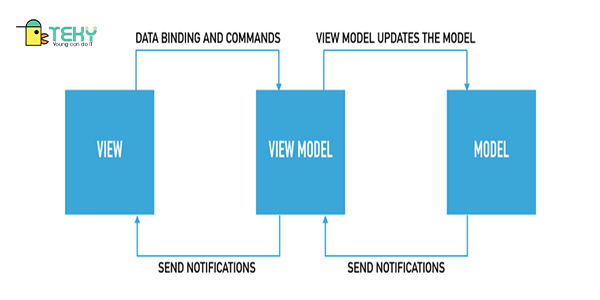
\includegraphics[width=0.67\textwidth]{images/mvvm.jpg}
  \caption{Mô hình kiến trúc MVVM \cite{tekyMVVM}.}
  \label{fig:fig18}
\end{figure}

    \begin{flushleft}
      \hspace*{0.8cm}Trong MVVM, thành phần Model vẫn giữ nguyên vai trò như trong kiến trúc MVC, tức là nơi lưu trữ dữ liệu cốt lõi và thực hiện các thao tác xử lý nghiệp vụ như gọi API, truy vấn cơ sở dữ liệu hoặc tính toán logic phức tạp. Tuy nhiên, điểm khác biệt nằm ở chỗ Model không tương tác trực tiếp với giao diện người dùng, mà tất cả dữ liệu sẽ được trung chuyển qua ViewModel. Nhờ vậy, việc tách rời trách nhiệm được thực hiện triệt để hơn, giúp hệ thống trở nên dễ kiểm soát và dễ kiểm thử hơn.
    \end{flushleft}

    \begin{flushleft}
      \hspace*{0.8cm}Trong khi đó, View trong kiến trúc MVVM chỉ đóng vai trò như một công cụ hiển thị, tương tự như trong MVC, nhưng điểm mạnh vượt trội nằm ở khả năng liên kết dữ liệu hai chiều (two-way data binding). Khi một người dùng nhập dữ liệu vào một thành phần như EditText, sự thay đổi này sẽ ngay lập tức được cập nhật vào ViewModel. Ngược lại, nếu dữ liệu trong ViewModel thay đổi – chẳng hạn do Model vừa nhận dữ liệu mới từ server – thì View cũng sẽ được cập nhật một cách tự động mà không cần lập trình viên can thiệp thêm. Nhờ vào cơ chế tự động này, lượng mã xử lý sự kiện và cập nhật giao diện giảm đáng kể, đồng thời làm giảm nguy cơ xảy ra lỗi do cập nhật thủ công.
    \end{flushleft}

    \begin{flushleft}
      \hspace*{0.8cm}Thành phần trung gian – ViewModel – chính là điểm khác biệt lớn nhất và mạnh mẽ nhất trong kiến trúc MVVM. ViewModel không chỉ chịu trách nhiệm chuẩn bị và cung cấp dữ liệu cho View, mà còn đóng vai trò là nơi lưu trữ trạng thái giao diện, đảm bảo tính nhất quán giữa các phiên làm việc hoặc khi xoay màn hình. Thêm vào đó, ViewModel có thể sử dụng các đối tượng LiveData hoặc StateFlow để cho phép View quan sát sự thay đổi của dữ liệu theo thời gian thực \cite{stateflow}. Điều này đặc biệt hữu ích trong các ứng dụng có giao diện phức tạp hoặc cần cập nhật liên tục, chẳng hạn như ứng dụng thương mại điện tử, mạng xã hội hoặc theo dõi vị trí.
    \end{flushleft}

    \begin{flushleft}
      \hspace*{0.8cm}Một lợi thế rõ rệt của MVVM so với MVC chính là mức độ giảm phụ thuộc giữa các thành phần, từ đó giúp hệ thống linh hoạt hơn khi mở rộng hoặc thay đổi một phần cụ thể. Do View và Model không còn liên kết trực tiếp, nên việc thay đổi cấu trúc giao diện hoặc định dạng dữ liệu trong Model sẽ không gây ảnh hưởng đến phần còn lại của hệ thống. Đồng thời, với sự hỗ trợ mạnh mẽ từ Jetpack (Android Architecture Components), việc triển khai MVVM trên Android trở nên thuận tiện hơn bao giờ hết nhờ các thư viện tích hợp như ViewModel, LiveData, Room và Data Binding.
    \end{flushleft}

    \begin{flushleft}
      \hspace*{0.8cm}Tóm lại, MVVM không chỉ là một bước tiến tự nhiên từ MVC mà còn là một kiến trúc phù hợp với xu hướng phát triển hiện đại – nơi giao diện cần phản hồi nhanh chóng, dữ liệu cập nhật liên tục và nhóm phát triển cần phối hợp hiệu quả. Nhờ khả năng tự động cập nhật giao diện khi dữ liệu thay đổi, giảm thiểu mã lặp, cũng như tăng khả năng kiểm thử và tái sử dụng mã nguồn, kiến trúc MVVM đã và đang trở thành lựa chọn ưu tiên trong các dự án Android có quy mô trung bình đến lớn, nơi yêu cầu về hiệu suất và khả năng mở rộng ngày càng được đặt lên hàng đầu.
    \end{flushleft}

% 4.4
\subsection{Kiến trúc Client/Server}
\renewcommand{\labelitemi}{--}    
    \begin{flushleft}
        \hspace*{0.8cm}Trong bối cảnh số hóa mạnh mẽ hiện nay, nơi mà hầu hết các ứng dụng đều cần tương tác và trao đổi dữ liệu với hệ thống bên ngoài thông qua Internet, kiến trúc Client/Server đã trở thành một nền tảng không thể thiếu trong thiết kế hệ thống phần mềm hiện đại. Đặc biệt, với các ứng dụng yêu cầu đồng bộ dữ liệu liên tục, cập nhật thông tin theo thời gian thực hoặc sử dụng tài nguyên được lưu trữ trên máy chủ từ xa, mô hình Client/Server đóng vai trò cốt lõi trong việc đảm bảo quá trình trao đổi dữ liệu diễn ra mượt mà, chính xác và có khả năng mở rộng cao. Tuy nhiên, để phát huy tối đa hiệu quả, kiến trúc Client/Server thường được sử dụng kết hợp với các kiến trúc nội bộ như MVC hoặc MVVM nhằm tách biệt rõ ràng giữa xử lý logic, giao diện người dùng và việc giao tiếp với hệ thống bên ngoài, từ đó giúp quá trình phát triển ứng dụng trở nên rõ ràng, có cấu trúc và dễ bảo trì hơn.
    \end{flushleft}

    \begin{flushleft}
      \hspace*{0.8cm}Về bản chất, kiến trúc Client/Server mô tả mô hình trong đó có sự phân chia rõ ràng giữa hai vai trò chính: Client (ứng dụng phía người dùng) và Server (máy chủ xử lý trung tâm). Trong mô hình này, các thiết bị đầu cuối như điện thoại, máy tính bảng hay trình duyệt web sẽ đóng vai trò là Client – nơi người dùng thực hiện các thao tác như gửi yêu cầu truy vấn dữ liệu, cập nhật thông tin cá nhân hoặc thao tác với giao diện ứng dụng. Những yêu cầu này, thường được gửi đi thông qua các giao thức phổ biến như HTTP, HTTPS hoặc WebSocket, sẽ được máy chủ tiếp nhận, xử lý và phản hồi tương ứng. Máy chủ, tức Server, sẽ tiếp nhận request từ Client, thực hiện các tác vụ cần thiết như truy xuất cơ sở dữ liệu, xử lý logic nghiệp vụ hoặc tính toán nâng cao, rồi trả lại kết quả phù hợp dưới dạng dữ liệu (thường là JSON hoặc XML).
    \end{flushleft}

        % https://codelearn.io/sharing/tim-hieu-ve-mo-hinh-client-server
\begin{figure}[H]
  \centering
  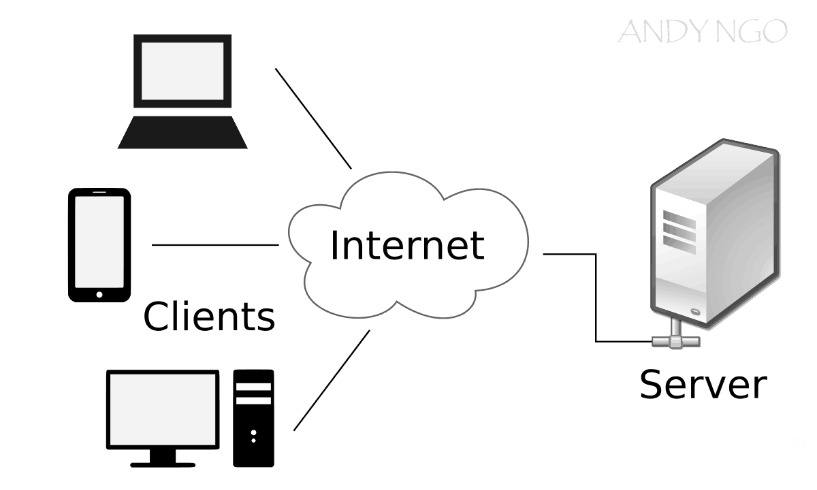
\includegraphics[width=0.75\textwidth]{images/client-server.jpg}
  \caption{Mô hình Client – Server \cite{codelearnClientServer}.}
  \label{fig:fig17}
\end{figure}

    \begin{flushleft}
      \hspace*{0.8cm}Một điểm quan trọng trong kiến trúc Client/Server là tính phân tán và độc lập giữa hai thành phần. Trong khi Client tập trung vào trải nghiệm người dùng như hiển thị giao diện, điều hướng màn hình, thu thập và hiển thị dữ liệu, thì Server lại tập trung vào việc xử lý các logic phức tạp, đảm bảo tính nhất quán của dữ liệu, bảo mật truy cập, và cung cấp tài nguyên theo cách tối ưu nhất. Mối quan hệ giữa Client và Server là một mối quan hệ chặt chẽ nhưng độc lập: mỗi bên có thể được nâng cấp hoặc thay đổi mà không ảnh hưởng trực tiếp đến bên còn lại, miễn là giao diện lập trình ứng dụng (API) giữa hai bên vẫn được tuân thủ nhất quán. Nhờ sự phân chia nhiệm vụ rõ ràng này, hệ thống có thể dễ dàng mở rộng về quy mô, nâng cấp từng thành phần riêng biệt và tối ưu hiệu suất xử lý.
    \end{flushleft}

    \begin{flushleft}
      \hspace*{0.8cm}Kiến trúc Client/Server thể hiện rõ vai trò trung tâm trong nhiều loại ứng dụng hiện đại có quy mô người dùng lớn, chẳng hạn như mạng xã hội (Facebook, Instagram) \cite{social-apps}, ứng dụng ngân hàng (Vietcombank, BIDV SmartBanking), thương mại điện tử (Shopee, Tiki), hay các nền tảng học trực tuyến (Google Classroom, Coursera). Trong các ứng dụng này, Client đóng vai trò là công cụ trung gian cho người dùng truy cập dịch vụ, trong khi Server xử lý các yêu cầu như xác thực tài khoản, truy xuất đơn hàng, hoặc cung cấp nội dung bài giảng. Đặc biệt, với nhu cầu chia sẻ dữ liệu đồng bộ giữa nhiều thiết bị khác nhau, kiến trúc Client/Server cho phép dữ liệu luôn được lưu trữ tập trung trên máy chủ, đảm bảo tính nhất quán và khả năng truy cập mọi lúc, mọi nơi.
    \end{flushleft}

    \begin{flushleft}
      \hspace*{0.8cm}Tóm lại, kiến trúc Client/Server không chỉ đơn thuần là mô hình truyền thống trong phát triển phần mềm mà còn là nền tảng quan trọng trong xây dựng các hệ thống hiện đại có khả năng mở rộng và tương tác mạnh mẽ. Khi được kết hợp hợp lý với các kiến trúc nội bộ như MVC hoặc MVVM, kiến trúc này mang lại khả năng tổ chức mã nguồn rõ ràng, giảm độ phức tạp, đồng thời tối ưu hóa hiệu suất và khả năng bảo trì của hệ thống phần mềm, đặc biệt là trong các ứng dụng di động kết nối Internet như hiện nay.
    \end{flushleft}